\documentclass[mathserif,8pt]{beamer}
\usepackage{indentfirst,mathrsfs}
\usepackage{amssymb}
\usepackage{pifont}
\usepackage{amsfonts}
\usepackage{booktabs}
\usepackage{color} 
\usepackage{bbm}
\usepackage{graphicx} 
\usepackage{indentfirst,mathrsfs}
\setbeamertemplate{footline}[frame number]

\usetheme{Darmstadt}

\usepackage{times}
\usefonttheme{structurebold}

\usepackage[english]{babel}
\usepackage{pgf,pgfarrows,pgfnodes,pgfautomata,pgfheaps}
\usepackage{amsmath,amssymb,mathrsfs}
\usepackage[latin1]{inputenc}
\usepackage{color}
\beamertemplatetextbibitems
\setbeamercovered{dynamic}



\definecolor{rgb0}{rgb}{1.0,0.5,0.5}
\definecolor{rgb1}{rgb}{0.0,0.5,0.5}
\definecolor{rgb2}{rgb}{0.8,0.6,0.6}
\definecolor{rgb3}{rgb}{0.1,0.7,0.6}

\newtheorem{property}{Property}

\newtheorem{construction}{Construction}
\newtheorem{proposition}{Proposition}




\pgfdeclaremask{tu}{beamer-tu-logo-mask}
\pgfdeclaremask{computer}{beamer-computer-mask}
\pgfdeclareimage[interpolate=true,mask=computer,height=2cm]{computerimage}{beamer-computer}
\pgfdeclareimage[interpolate=true,mask=computer,height=2cm]{computerworkingimage}{beamer-computerred}
\pgfdeclareimage[mask=tu,height=.5cm]{logo}{beamer-tu-logo}

\logo{\pgfuseimage{logo}}
\title{Research on Fast Algebraic Immunity}

\author{Liu Zhang}
\institute{Department of Computer Science, Shdantou University}
\colorlet{redshaded}{red!25!bg} \colorlet{shaded}{black!25!bg}
\colorlet{shadedshaded}{black!10!bg}
\colorlet{blackshaded}{black!40!bg}

\colorlet{darkred}{red!80!black} \colorlet{darkblue}{blue!80!black}
\colorlet{darkgreen}{green!80!black}

\def\radius{0.96cm}
\def\innerradius{0.85cm}

\def\softness{0.4}
\definecolor{softred}{rgb}{1,\softness,\softness}
\definecolor{softgreen}{rgb}{\softness,1,\softness}
\definecolor{softblue}{rgb}{\softness,\softness,1}

\definecolor{softrg}{rgb}{1,1,\softness}
\definecolor{softrb}{rgb}{1,\softness,1}
\definecolor{softgb}{rgb}{\softness,1,1}

\newcommand{\Bandshaded}[2]{
  \color{shadedshaded}
  \pgfmoveto{\pgfxy(-0.5,0)}
  \pgflineto{\pgfxy(-0.6,0.1)}
  \pgflineto{\pgfxy(-0.4,0.2)}
  \pgflineto{\pgfxy(-0.6,0.3)}
  \pgflineto{\pgfxy(-0.4,0.4)}
  \pgflineto{\pgfxy(-0.5,0.5)}
  \pgflineto{\pgfxy(4,0.5)}
  \pgflineto{\pgfxy(4.1,0.4)}
  \pgflineto{\pgfxy(3.9,0.3)}
  \pgflineto{\pgfxy(4.1,0.2)}
  \pgflineto{\pgfxy(3.9,0.1)}
  \pgflineto{\pgfxy(4,0)}
  \pgfclosepath
  \pgffill

  \color{black}
  \pgfputat{\pgfxy(0,0.7)}{\pgfbox[left,base]{#1}}
  \pgfputat{\pgfxy(0,-0.1)}{\pgfbox[left,top]{#2}}
}

\newcommand{\Band}[2]{
  \color{shaded}
  \pgfmoveto{\pgfxy(-0.5,0)}
  \pgflineto{\pgfxy(-0.6,0.1)}
  \pgflineto{\pgfxy(-0.4,0.2)}
  \pgflineto{\pgfxy(-0.6,0.3)}
  \pgflineto{\pgfxy(-0.4,0.4)}
  \pgflineto{\pgfxy(-0.5,0.5)}
  \pgflineto{\pgfxy(4,0.5)}
  \pgflineto{\pgfxy(4.1,0.4)}
  \pgflineto{\pgfxy(3.9,0.3)}
  \pgflineto{\pgfxy(4.1,0.2)}
  \pgflineto{\pgfxy(3.9,0.1)}
  \pgflineto{\pgfxy(4,0)}
  \pgfclosepath
  \pgffill

  \color{black}
  \pgfputat{\pgfxy(0,0.7)}{\pgfbox[left,base]{#1}}
  \pgfputat{\pgfxy(0,-0.1)}{\pgfbox[left,top]{#2}}
}

\newcommand{\BaenderNormal}
{%
  \pgfsetlinewidth{0.4pt}
  \color{black}
  \pgfputat{\pgfxy(0,5)}{\Band{input tapes}{}}
  \pgfputat{\pgfxy(0.35,4.6)}{\pgfbox[center,base]{$\vdots$}}
  \pgfputat{\pgfxy(0,4)}{\Band{}{}}

  \pgfxyline(0,5)(0,5.5)
  \pgfxyline(1.2,5)(1.2,5.5)
  \pgfputat{\pgfxy(0.25,5.25)}{\pgfbox[left,center]{$w_1$}}

  \pgfxyline(0,4)(0,4.5)
  \pgfxyline(1.8,4)(1.8,4.5)
  \pgfputat{\pgfxy(0.25,4.25)}{\pgfbox[left,center]{$w_n$}}
  \ignorespaces}

\newcommand{\BaenderZweiNormal}
{%
  \pgfsetlinewidth{0.4pt}
  \color{black}
  \pgfputat{\pgfxy(0,5)}{\Band{Zwei Eingabebader}{}}
  \pgfputat{\pgfxy(0,4.25)}{\Band{}{}}

  \pgfxyline(0,5)(0,5.5)
  \pgfxyline(1.2,5)(1.2,5.5)
  \pgfputat{\pgfxy(0.25,5.25)}{\pgfbox[left,center]{$u$}}

  \pgfxyline(0,4.25)(0,4.75)
  \pgfxyline(1.8,4.25)(1.8,4.75)
  \pgfputat{\pgfxy(0.25,4.5)}{\pgfbox[left,center]{$v$}}
  \ignorespaces}

\newcommand{\BaenderHell}
{%
  \pgfsetlinewidth{0.4pt}
  \color{black}
  \pgfputat{\pgfxy(0,5)}{\Bandshaded{input tapes}{}}
  \color{shaded}
  \pgfputat{\pgfxy(0.35,4.6)}{\pgfbox[center,base]{$\vdots$}}
  \pgfputat{\pgfxy(0,4)}{\Bandshaded{}{}}

  \color{blackshaded}
  \pgfxyline(0,5)(0,5.5)
  \pgfxyline(1.2,5)(1.2,5.5)
  \pgfputat{\pgfxy(0.25,5.25)}{\pgfbox[left,center]{$w_1$}}

  \pgfxyline(0,4)(0,4.5)
  \pgfxyline(1.8,4)(1.8,4.5)
  \pgfputat{\pgfxy(0.25,4.25)}{\pgfbox[left,center]{$w_n$}}
  \ignorespaces}

\newcommand{\BaenderZweiHell}
{%
  \pgfsetlinewidth{0.4pt}
  \color{black}
  \pgfputat{\pgfxy(0,5)}{\Bandshaded{Zwei Eingabebader}{}}%
  \color{blackshaded}
  \pgfputat{\pgfxy(0,4.25)}{\Bandshaded{}{}}
  \pgfputat{\pgfxy(0.25,4.5)}{\pgfbox[left,center]{$v$}}
  \pgfputat{\pgfxy(0.25,5.25)}{\pgfbox[left,center]{$u$}}%

  \pgfxyline(0,5)(0,5.5)
  \pgfxyline(1.2,5)(1.2,5.5)

  \pgfxyline(0,4.25)(0,4.75)
  \pgfxyline(1.8,4.25)(1.8,4.75)
  \ignorespaces}

\newcommand{\Slot}[1]{%
  \begin{pgftranslate}{\pgfpoint{#1}{0pt}}%
    \pgfsetlinewidth{0.6pt}%
    \color{structure}%
    \pgfmoveto{\pgfxy(-0.1,5.5)}%
    \pgfbezier{\pgfxy(-0.1,5.55)}{\pgfxy(-0.05,5.6)}{\pgfxy(0,5.6)}%
    \pgfbezier{\pgfxy(0.05,5.6)}{\pgfxy(0.1,5.55)}{\pgfxy(0.1,5.5)}%
    \pgflineto{\pgfxy(0.1,4.0)}%
    \pgfbezier{\pgfxy(0.1,3.95)}{\pgfxy(0.05,3.9)}{\pgfxy(0,3.9)}%
    \pgfbezier{\pgfxy(-0.05,3.9)}{\pgfxy(-0.1,3.95)}{\pgfxy(-0.1,4.0)}%
    \pgfclosepath%
    \pgfstroke%
  \end{pgftranslate}\ignorespaces}

\newcommand{\SlotZwei}[1]{%
  \begin{pgftranslate}{\pgfpoint{#1}{0pt}}%
    \pgfsetlinewidth{0.6pt}%
    \color{structure}%
    \pgfmoveto{\pgfxy(-0.1,5.5)}%
    \pgfbezier{\pgfxy(-0.1,5.55)}{\pgfxy(-0.05,5.6)}{\pgfxy(0,5.6)}%
    \pgfbezier{\pgfxy(0.05,5.6)}{\pgfxy(0.1,5.55)}{\pgfxy(0.1,5.5)}%
    \pgflineto{\pgfxy(0.1,4.25)}%
    \pgfbezier{\pgfxy(0.1,4.25)}{\pgfxy(0.05,4.15)}{\pgfxy(0,4.15)}%
    \pgfbezier{\pgfxy(-0.05,4.15)}{\pgfxy(-0.1,4.2)}{\pgfxy(-0.1,4.25)}%
    \pgfclosepath%
    \pgfstroke%
  \end{pgftranslate}\ignorespaces}

\newcommand{\ClipSlot}[1]{%
  \pgfrect[clip]{\pgfrelative{\pgfxy(-0.1,0)}{\pgfpoint{#1}{4cm}}}{\pgfxy(0..2,1.5)}\ignorespaces}

\newcommand{\ClipSlotZwei}[1]{%
  \pgfrect[clip]{\pgfrelative{\pgfxy(-0.1,0)}{\pgfpoint{#1}{4.25cm}}}{\pgfxy(0.2,1.25)}\ignorespaces}


\AtBeginSection[]{\frame{\frametitle{Outline}\tableofcontents[current]}}
\begin{document}

\frame{\titlepage}

%\part{Main Part}
%\frame{\frametitle{Outline}\tableofcontents[part=1]}

\section{Self Introduction}
\frame { \frametitle{Self Instruction}
\textbf{Educational Background}
	\begin{itemize}
	\item  2013.9-2017.6 Xinyang Normal University, College of Computer and Information Technology
	\item  2017.9-now Shantou University, College of Engineering
	\end{itemize}
\textbf{Academic Research Achievements}
	\begin{itemize}
		\item  	Chen Yindong, \textbf{Zhang Liu}, Tang Deng, Cai Weihong. Translation Equivalence of Boolean Functions Expressed by Primitive Element. IEICE Transaction Fundamentals, 2019, 4: 672-675.
		
		\item 	Chen Yindong, \textbf{Zhang Liu}, and Xu jianlong, Cai Weihong. A Lower Bound of Fast Algebraic Immunity of A Class of 1-Resilient Boolean Functions. IEEE ACCESS,2019, 12:90145-90151.
		
	    \item	Chen Yindong, \textbf{Zhang Liu}, and Guo Fei , Cai Weihong. Fast algebraic immunity of $2^{m}+2$ \& $2^{m}+3$ variables majority function. IEEE ACCESS,2019,12:80733-80736.

	\end{itemize}
}
\section{Translation Equivalence of Boolean Functions \protect \\ Expressed By Primitive Element}

\frame { \frametitle{Instruction}
	
	\begin{figure}[h]
		\centering  
		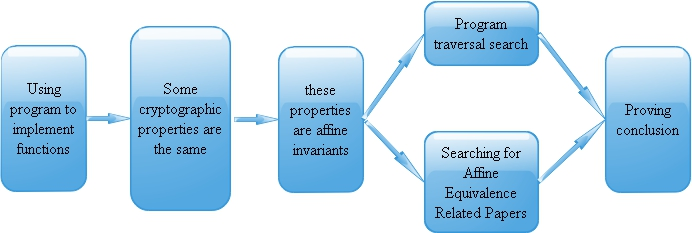
\includegraphics[width=1.0\linewidth]{translate-equivalation.jpg}  
	%	\caption{Research process}  
	\end{figure}
}


\frame { \frametitle{Preliminaries}
	\begin{itemize}
		\item The sequence $\{s_t{}\}$ obey the recursion $\sum_{j=0}^{n}m_{j}s_{t+j}=0,m_{j}\in F_{2}$
		\item $m(x)=1+m_{1}x+\cdots+m_{n-1}x^{n-1}+x^{n}$
		\item The generator matrix of the sequence  
		$$    M=
		\left(
		\begin{array}{ccccc}
		0 & 1 & \cdots & 0 & 0 \\
		0 & 0 & \cdots & 0 & 0\\
		\cdots & \cdots & \cdots & \cdots & \cdots\\
		0 & 0 & \cdots & 0 & 1\\
		m_{0} & m_{1} & \cdots &m_{n-2} & m_{n-1}\\
		\end{array}
		\right).
		$$
		
		\item $(s_{t+1},s_{t+2},...,s_{t+n})^{T}=M(s_{t},s_{t+1},...,s_{t+n-1})^{T}
		=M^{t+1}(s_{0},s_{1},...,s_{n-1})^{T} $
		
		\item If the initial state of the register is $b$, $S=(b,Mb,...,M^{q-2}b)$.
		\item Let $b_{0}=(1,0,...,0)^{T}$, $S_{k}=(M^{k}b_{0},M^{k+1}b_{0},...,M^{k+q-2}b_{0}),$ where $0\leq k\leq q-2$.
		
		\item  $1_{f}=\{M_{j}^{i_{1}}b_{0},M_{j}^{i_{2}}b_{0},...,M_{j}^{i_{w}}b_{0}\},$ where $0\leq i_{1}< i_{2}<...< i_{w}\leq q-2.$
	\end{itemize}
}


\frame { \frametitle{Translation equivalence relation of support of C-F function}
	 \begin{construction}[1]\cite{Carlet2008}
		Let n be an integer greater than 1 and $\alpha$ be a primitive element of $F_{2^{n}}$. If $f$ is an $n$-variable Boolean function whose support is $$\{\textbf{0},\alpha^{s},\alpha^{s+1},...,\alpha^{s+2^{n-1}-2}\},$$where $0\leq s<2^{n}-1$ is an integer, then $f$ has optimal algebraic immunity $\lceil n/2\rceil$.
	\end{construction}
	~ \\
	\begin{construction}[2]\cite{Wang2010Constructions}
	Let n be an integer greater than 1 and $\underline{s}=(s_{t})_{t\geq 0}$ be an $m$-sequence of order n. If an $n$-variable Boolean function $f$ whose support is
	$$\{\textbf{0}\} \cup \{s_{t},s_{t+1},...,s_{t+n-1}|0\leq t \leq 2^{n-1}-2\},$$
	where \textbf{0} denotes the all-zero vector in $F_{2}^{n}$, then $f$ has optimal algebraic immunity  $\lceil n/2\rceil$.
	\end{construction}
}

\frame { \frametitle{Translation equivalence relation of support of C-F function}
 

	\begin{lemma}[1]\cite{Chen2013}
	Let n be an integer greater than 1 and $m(x)$ be a primitive polynomial of degree n over $F_{2}$. If $\alpha \in F_{2^{n}}$ is a root of $m(x)$ and $\underline{s}=(s_{t})_{t\geq 0} \in G(m(x))$ is a nonzero sequence, then there exists a basis $\{\beta_{0},\beta_{1},...,\beta_{n-1}\}$ of $F_{2^{n}}$ such that
	$$s_{t}\beta_{0}\oplus s_{t+1}\beta_{1}\oplus \cdots \oplus
	s_{t+n-1}\beta_{n-1}=\alpha^{t},t \geq 0. $$
	\end{lemma}
	~ \\
	\begin{lemma}[2]\cite{Wang2010}
	Let $f\in Bn$ and
	$$1_{f}=\{M_{1}^{k_{1}+i_{1}}b_{0},M_{1}^{k_{1}+i_{2}}b_{0},...,M_{1}^{k_{1}+i_{w}}b_{0}\},$$where $M_{1}$ is the generator matrix of the sequence and $0\leq i_{1}<i_{2}<...<i_{w}\leq q-2$. Clearly, any $g \sim f$ can be represented by
	$$1_{g}=\{M_{j}^{k_{2}+i_{1}}b_{0},M_{j}^{k_{2}+i_{2}}b_{0},...,M_{j}^{k_{2}+i_{w}}b_{0}\},$$ where $1\leq j \leq \phi(q-1)/n$, $M_{j}$ is a generator matrix and $0 \leq k_{2} \leq q-2 $.
	\end{lemma}
}

\frame { \frametitle{Translation equivalence relation of support of C-F function}
	\begin{theorem}[1]
		Let n be an integer greater than 1 and $\alpha$ be a primitive element of $F_{2^{n}}$. If $f$ is an $n$-variable Boolean function whose support is $$\{0,\alpha^{s},\alpha^{s+1},...,\alpha^{s+2^{n-1}-2}\},$$where $0\leq s<2^{n}-1$ is an integer. When s takes different values, Boolean functions obtained are affine equivalent.
		
	\end{theorem}
	 
	$$M^{t}b_{0}\beta_{0}\oplus M^{t+1}b_{0}\beta_{1}\oplus\cdots\oplus M^{t+n-1}b_{0}\beta_{n-1}=\alpha^{t},t\geq 0.$$
	$$1_{f}=\{0\}\cup\{M_{1}^{i+s}b_{0}|i=0,1,...,2^{n-1}-2,0\leq s<2^{n}-1\}.$$ 
	$$1_{f_{1}}=\{M_{1}^{i}b_{0}|i=0,1,...,2^{n-1}-1\}.$$  
	$$1_{g}=\{M_{1}^{s+i}b_{0}|i=0,1,...,2^{n-1}-1\}$$
}

\frame { \frametitle{Translation equivalence relation of support of Tu-Deng function and T-C-T function}
	
	\begin{theorem}[2]
		Let $n=2k$ and $\alpha$ be a primitive element of $F_{2^{k}}$. The Boolean function $g:F_{2^{k}}\rightarrow F_{2}$ is defined as
		$$supp(g)=\{1=\alpha^{s},\alpha^{s+1},...,\alpha^{2^{k-1}+s-1}\}.$$ Let Boolean function $f:F_{2^{k}}\times F_{2^{k}}\rightarrow F_{2}$ be defined as
		$$f(x,y)=g(x/y).$$the support of Boolean function $f$ can be written
		$$supp(f)=\{\beta^{(2^{k}+1)(i+s)}+\beta^{2^{k}-1}\cdot\beta^{(2^{k}+1)j}\},$$where $i\in(0,2^{k}),j\in(0,2^{k}),(i-j)\pmod{2^{k}-1}\in(0,2^{k-1}-1)$, $0\leq s<2^{k}-1$ is an integer.
	\end{theorem}
}

\frame { \frametitle{Translation equivalence relation of support of Tu-Deng function and T-C-T function}

	\begin{theorem}[3]
		Let $n=2k>4$. Let  $\alpha$ be a primitive element of the finite field $F_{2^{k}}$. Set $\Delta=\{\alpha^{s},...,\alpha^{2^{k-1}+s-1}\}$ where $0\leq s<2^{k}-1$ is an integer. Then Boolean function $f\in B_{n}$ as follows:$$f(x,y)=g(xy),$$ where the support of Boolean function g is $\Delta$.the support of Boolean function $f$ can be written
		$$supp(f)=\{\beta^{(2^{k}+1)(i+s)}+\beta^{2^{k}-1}\cdot\beta^{(2^{k}+1)j}\},$$where $i\in(0,2^{k}),j\in(0,2^{k}),(i+j)\pmod{2^{k}-1}\in(0,2^{k-1}-1)$, $0\leq s<2^{k}-1$ is an integer.
	\end{theorem}

	\begin{theorem}[4]
		When s takes different values, T-C-T functions are affine equivalent.
		Meanwhile, Tu-Deng function are also affine equivalent.
	\end{theorem}

}


\section{A Lower Bound of Fast Algebraic Immunity of \protect \\ A Class of 1-Resilient Boolean Functions  }
\frame{\frametitle{Instruction}
	\begin{figure}[h]
		\centering  
		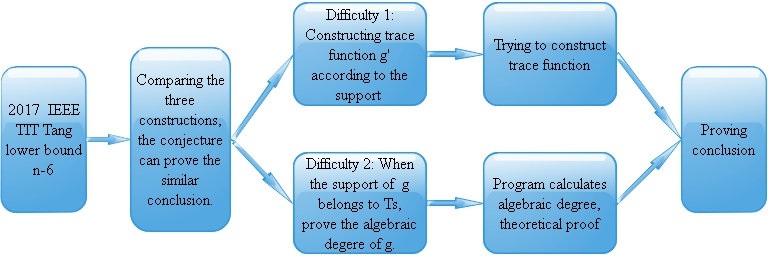
\includegraphics[width=1.0\linewidth]{n-6.jpg}  
	%	\caption{Research process}  
	\end{figure}

	
}

\frame{\frametitle{Preliminaries}
	\begin{definition}[1]\cite{Meier2004}
		The algebraic immunity of a Boolean function $f\in \mathcal{B}_{n}$, expressed by $AI(f)$, is defined as
		$AI(f)=\min\{\deg(g)|fg=0 \ or \ (f+1)g=0,g\neq0 \in \mathcal{B}_{n}\}.$
	\end{definition}

	~ \\ 
	
	\begin{definition}[2]\cite{Liu2009fast}
		The fast algebraic immunity of a Boolean function $f\in \mathcal{B}_n$, expressed by $FAI(f)$, is defined as
		$FAI(f)=\min\{ 2AI(f), \min\{\deg(g)+\deg(fg)|1\le \deg(g)<AI(f)\}\}.$
	\end{definition}
}

\frame{\frametitle{A lower bound of fast algebraic immunity of a class of 1-resilient Boolean functions}
	\begin{construction}[1]\cite{Tang2014}
		Let $ n=2k\ge 10 $, $\alpha$ be a primitive element of the finite field $\mathbb{F}_{2^{k}}$. Let $\Delta_{s}=\{s,s+1,\cdots,s+2^{k-1}-1\}$ and $\overline{\Delta_{s}}=\mathbb{Z}_{2^{k}-1}  \backslash \Delta_{s}$ where $0\le s <2^{k-1}-1$. Boolean Function $f_{s}\in \mathcal{B}_n$ can be defined as:
		$$f_{s}(x,y)=b_{s}(x,y)+u_s(x,y) \eqno(1)$$ where $b_{s}(x,y)\in \mathcal{B}_n$ belongs to (2) and  $supp(u_{s})$ includes the following three parts:
		\begin{itemize}
			
			\item   $\{(\alpha^{i},\alpha^{s+2^{k-1}-i-1})\ | \ i\in \{0,\cdots,s+2^{k-1}-1\} \}  \cup \{(\alpha^{i},\alpha^{s-i-1})\ | \ s >i \in \overline{\Delta_{s}} \}$
			
			\item  $\{(0,\alpha^{i})\ | \ i \in \Delta_{s}\}$
			\item  $\{(\alpha^{i},0)\ | \ i \in \Delta_{s}\}$
		\end{itemize}		
	\end{construction} 	

	\begin{theorem}[1]\cite{Tang2014}
		Let $n=2k$, $f_{s}$ be the $n$-variable Boolean function in Construction 1. Then algebraic immunity of Boolean function $f_{s}$ is $k$, i.e., $AI(f_{s})=k$.
	\end{theorem}

	
}


\frame{\frametitle{A class of Boolean functions with almost optimal algebraic immunity}
	\begin{construction}[2]\cite{Tang2013}
		Let  $ n=2k\ge 4$, $\alpha$ be a primitive element of the finite field $\mathbb{F}_{2^{k}}$ and $\Delta_{s}=\{s,s+1, \cdots, s+2^{k-1}-1\}$ where $0\le s<2^{k}-1$. Boolean function $b_{s}(x,y)\in \mathcal{B}_n$ can be defined as:$$b_{s}(x,y)=g_{s}(xy) \eqno(2)$$
		where $g_{s}$ is defined on $\mathbb{F}_{2^{k}}$ with $supp(g_{s})=\{\alpha^{i}\ | \ i\in \Delta_{s} \}$.
	\end{construction}
	~ \\
	\begin{proposition}[1]\cite{Tang2013}
		The $n$-variable Boolean function $b_{s}(x,y)$ in Construction 2 includes the four cryptographic properties where  $0\le s<2^{k}-1$:
		
		
		1) $AI(b_{s})=k$;

		2) $FAI(b_{s})\ge n-2$.
		
	\end{proposition}
	
}

\frame{\frametitle{A lower bound of fast algebraic immunity of a class of 1-resilient Boolean functions}
	
	\begin{theorem}[2]
		Let $n=2k>10$, $0\le s<2^{k-1}-1$, then the FAI of $f_{s}$ in Construction 1 is at least $n-6$.
	\end{theorem}
	
	\begin{proof}
		Assume  $\deg(g)+\deg(f_{s}g)\le n-7.$  $$f_{s}g=(b_{s}+u_{s})g \eqno(3)$$
		\begin{itemize}
			\item $supp(g) \subseteq T_{s}$
			
			\item $supp(g) \nsubseteq T_{s}$,$g'(x,y)=tr_{1}^{k}(z'\alpha^{2^{k-1}-s}xy+r'\alpha^{2^{k}-s}xy)$
			$$f_{s}gg'=(b_{s}+u_{s})gg'=(b_{s}+u_{s})g'g=b_{s}gg'$$ $g'$ is a nonzero annihilator of $u_{s}$.  $$\deg(gg')+\deg(f_{s}gg')=\deg(gg')+\deg(b_{s}gg')\le FAI(f_{s})+4\le n-3.$$
		\end{itemize}
		
	\end{proof}
}

\frame{\frametitle{A lower bound of fast algebraic immunity of a class of 1-resilient Boolean functions}
	
	
	\begin{lemma}[1]
		Let  $ n=2k \ge 10$, $\alpha$ be a primitive element of the finite filed $\mathbb{F}_{2^{k}}$. Let $T_{s}=\{(x,0)\ | \ x \in F_{2^{k}} \} \cup \{(0,y)\ | \ y \in \mathbb{F}_{2^{k}} \}\cup
		\{(z,\alpha^{s+2^{k-1}-1}z^{2^{k}-2})\ | \ z \in \mathbb{F}_{2^{k}}^{*}\} \cup
		\{(z,\alpha^{s-1}z^{2^{k}-2})\ | \ z \in \mathbb{F}_{2^{k}}^{*}\}$ where $0\le s<2^{k-1}-1$. When $g\in \mathcal{B}_n$ has $supp(g) \subseteq T_{s}$, $\deg(g)\ge k-1$.
		
	\end{lemma}
	
	\begin{construction}[2] Let $ n=2k\ge 4$, $\alpha$ be a primitive element of the finite field $\mathbb{F}_{2^{k}}$. Let $\Delta_{m}=\{m+2,m+3,\cdots,m+2^{k-1}-1\}$ where $0\le m<2^{k}-1$. Boolean function $b_{m}(x,y)\in \mathcal{B}_n$ can be defined as:$$b_{m}(x,y)=g_{m}(xy) \eqno(4)$$
		where $g_{m}$ is defined on $\mathbb{F}_{2^{k}}$ with $supp(g_{m})=\{\alpha^{j}\ | \ j\in \Delta_{m} \}$.
	\end{construction}
	
	\begin{theorem}[3]
		Let $f$ be the $2k$-variable Boolean function in Construction 2. Then, $AI(f)$ is $k-1$.
	\end{theorem}
}


\frame{\frametitle{A class of Boolean functions with almost optimal algebraic immunity}

	\begin{lemma}[2]\cite{JinQ2011}
		For $k\ge{3},\  1 \le t \le 2^k-2$, let
		
		\begin{equation*}
		M_{\le k-1,\ t} = \left \{(a,b)\in \mathbb{Z}^2 | \begin{split}      &    \ \ \ 0 \le a,b \le 2^{k}-2, \\
		&    {a-b} \equiv{t}\pmod {2^{k}{-}1}, \\
		&    wt(\overline{a})+wt(\overline{b}) \le{k-1}
		\end{split}
		\right\}.
		\end{equation*}
		Then $|M_{\le k-1,\ t}|\le{2^{k-1}-1}$.
	\end{lemma}
	
	
	\begin{lemma}[3]
		For $k\ge{3},\  1 \le t \le 2^k-2$, let
		\begin{equation*}
		M_{k-1,\ t} = \left \{(a,b)\in \mathbb{Z}^2  | \begin{split}      &    \ \ \ 0 \le a,b \le 2^{k}-2, \\
		&    {a-b} \equiv{t}\pmod {2^{k}{-}1}, \\
		&    wt(\overline{a})+wt(\overline{b}) = {k-1}
		\end{split}
		\right\}.
		\end{equation*}
		Then $|M_{k-1,\ t}|\ge 1$.
	\end{lemma}
	
}

\frame{\frametitle{A class of Boolean functions with almost optimal algebraic immunity}
	\begin{lemma}[4]
		For $k\ge{3},\  1 \le t \le 2^k-2$, let
		\begin{equation*}
		M_{\le k-2,\ t} = \left \{(a,b)\in \mathbb{Z}^2  | \begin{split}      &    \ \ \ 0 \le a,b \le 2^{k}-2, \\
		&    {a-b} \equiv{t}\pmod {2^{k}{-}1}, \\
		&    wt(\overline{a})+wt(\overline{b}) \le {k-2}
		\end{split}
		\right\}.
		\end{equation*}
		Then $|M_{\le k-2,\ t}| \le 2^{k-1}-2$.
		
	\end{lemma}
	
	\begin{lemma}[5]
		For $k\ge{3},\  t=0$, let
		\begin{equation*}
		M_{\le k-2,\ 0} = \left \{(a,b)\in \mathbb{Z}^2  | \begin{split}      &    \ \ \ 0 \le a,b \le 2^{k}-2, \\
		&    {a-b} \equiv{t}\pmod {2^{k}{-}1}, \\
		&    wt(\overline{a})+wt(\overline{b}) \le {k-2}
		\end{split}
		\right\}.
		\end{equation*}
		Then $|M_{\le k-2,\ 0}| \le 2^{k-1}-2$.
	\end{lemma}
}

\frame{\frametitle{A class of Boolean functions with almost optimal algebraic immunity}
	\begin{lemma}[6]
		For $k\ge{3},\ 0 \le t \le 2^k-2$, let
		\begin{equation*}
		M_{\le k-2,\ t} = \left \{(a,b)\in \mathbb{Z}^2 | \begin{split}      &    \ \ \ 0 \le a,b \le 2^{k}-2, \\
		&    {a-b} \equiv{t}\pmod {2^{k}{-}1}, \\
		&    wt(\overline{a})+wt(\overline{b}) \le {k-2}
		\end{split}
		\right\}.
		\end{equation*}
		Then $|M_{\le k-2,\ t}| \le 2^{k-1}-2$.
		
	\end{lemma}
	
	\begin{lemma}[7]
		Let $ n=2k$, $\alpha$ be a primitive element of $\mathbb{F}_{2^{k}}$. Let $T_{s}=\{(0,y)\ | \ y \in \mathbb{F}_{2^{k}} \}\cup \{(x,0)\ | \ x \in \mathbb{F}_{2^{k}} \}\cup
		\{(\gamma,\alpha^{s+2^{k-1}-1}\gamma^{2^{k}-2})\ | \ \gamma \in \mathbb{F}_{2^{k}}^{*}\}\cup
		\{(\gamma,\alpha^{s-1}\gamma^{2^{k}-2})\ | \ \gamma \in \mathbb{F}_{2^{k}}^{*}\}$ where $0\le s<2^{k-1}-1$ and $U'=\{z\in \mathbb{F}_{2^{k}}^{*}\ | \ tr_{1}^{k}(z)=0\}$. For $0\le s<2^{k-1}-1$, if an arbitary element $(a,b)\in \mathbb{F}_{2^{k}}\times \mathbb{F}_{2^{k}}\backslash T_{s}$, there are $2(2^{k-2}(2^{k-2}-1))$  pair $(z',r')$ where $z',r'\in U'$ such that $g'(x,y)=tr_{1}^{k}(z'\alpha^{2^{k-1}-s}xy+r'\alpha^{2^{k}-s}xy)$ equals $1$ if $(x,y)=(a,b)$.
	\end{lemma}
	
	
}
\frame{\frametitle{A lower bound of fast algebraic immunity of a class of 1-resilient Boolean functions}
	
	\begin{theorem}[2]
		Let $n=2k>10$, $0\le s<2^{k-1}-1$, then the FAI of $f_{s}$ in Construction 1 is at least $n-6$.
	\end{theorem}
	
	\begin{proof}
		Assume  $\deg(g)+\deg(f_{s}g)\le n-7.$  $$f_{s}g=(b_{s}+u_{s})g \eqno(3)$$
		\begin{itemize}
			\item $supp(g) \subseteq T_{s}$
			
			\item $supp(g) \nsubseteq T_{s}$,$g'(x,y)=tr_{1}^{k}(z'\alpha^{2^{k-1}-s}xy+r'\alpha^{2^{k}-s}xy)$
			$$f_{s}gg'=(b_{s}+u_{s})gg'=(b_{s}+u_{s})g'g=b_{s}gg'$$ $g'$ is a nonzero annihilator of $u_{s}$.  $$\deg(gg')+\deg(f_{s}gg')=\deg(gg')+\deg(b_{s}gg')\le FAI(f_{s})+4\le n-3.$$
		\end{itemize}
		
	\end{proof}
}

\section{Fast Algebraic Immunity of $2^m+2$ \& $2^m+3$ \protect \\ Variables Majority Function}

\frame {\frametitle{Instruction}
	\begin{figure}[h]
		\centering  
		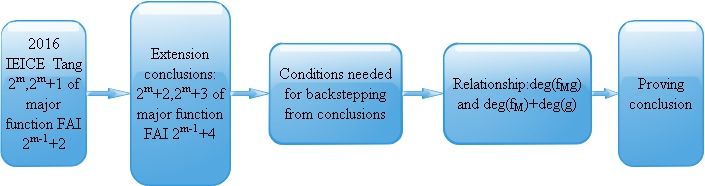
\includegraphics[width=1.0\linewidth]{exact-fai.jpg}  
	%	\caption{Research process}  
	\end{figure}


}
\frame {\frametitle{Preliminaries}


	\begin{definition}[1]\label{def:majf}\cite{Ding1991}
		The majority function is defined as
		\[f_M(x)=\begin{cases}
		1, & wt(x)\geq\left\lceil\frac{n}{2}\right\rceil \\
		0, &\mathrm{otherwise}.
		\end{cases}\]
	\end{definition}
	
	
	~ \\ 
	
	\begin{lemma}[1]\cite{Dalai2006}
		Let $f_M \in \mathcal{SB}_n$ be the majority function, then
		\begin{enumerate}[i)]
			\item $\deg(f_M)=2^{\lfloor \log_2n \rfloor}$;
			\item $AI(f_M) = \lceil\frac{n}{2}\rceil$.
		\end{enumerate}
	\end{lemma}

}


\frame {\frametitle{Main Result}
	
	\begin{theorem}[1]
		Let $f_M \in \mathcal{SB}_n$ be the majority function with $n \in \{2^m+2, 2^m+3\}$ where $m \ge 2$. Then $FAI(f_M)=2^{m-1}+4$.
	\end{theorem}

	\begin{lemma}[2]\cite{Armknecht2006}\label{upboundlemma}
		Let $n\ge2$, $f_M$ is the $n$-variable majority function .
		There are Boolean Functions $g$ and $h$ so that $f_Mg=h$ with  $d=\deg(h)=\lfloor n/2\rfloor+1$ and $e=\deg(g)=d-2^j$ where $j$ is the maximum number ensure that $e>0$.
	\end{lemma}

	\begin{lemma} [3]
		Let $f_M \in \mathcal{SB}_n$ be the majority function with $2^m+2 \le n < 2^{m+1}$ where $m \ge 2$. Then $FAI(f_M) \ge \lfloor \frac{n}{2} \rfloor + 3$.
	\end{lemma}
	
}

\frame {\frametitle{Main Result}	
	\begin{lemma}[4]
		Let $2^m+2 \le n < 2^{m+1}$ with $m \ge 2$ and $f_M \in \mathcal{SB}_n$ be the majority function.
		Let $A=\min\{\deg(h)|0 \ne h \in Ann(f_M)\}$. Then $FAI(f_M) \ge A+2 \ge AI(f_M)+2$.
	\end{lemma}
	~ \\
	\begin{proof}
		\begin{equation}\label{formula:unequal1}
		\begin{split}
		\min_{1 \le \deg(g) < AI(f_M+1)}\{\deg(g)+ \deg(   &   (f_M+1)g)\} \\
		&   \ge A+2\ge AI(f_M)+2
		\end{split}
		\end{equation}
	\end{proof}


}

\frame {\frametitle{Main Result}	

	\begin{lemma}[5]\rm \label{degplus1}
		Let $2^m+2 \le n < 2^{m+1}$ with $m \ge 2$ and $f_M \in \mathcal{SB}_n$ be the majority function.
		For any $n$-variable Boolean function $g$ with $\deg(g)=1$, then $\deg(f_M g)=\deg(f_M)+1$.
	\end{lemma}
	
	~ \\
 	\begin{theorem}[1]
 		Let $f_M \in \mathcal{SB}_n$ be the majority function with $n \in \{2^m+2, 2^m+3\}$ where $m \ge 2$. Then $FAI(f_M)=2^{m-1}+4$.
 	\end{theorem}
}

\frame {\frametitle{Sequential Studies}	
	
	\begin{figure}[h]
		\centering  
		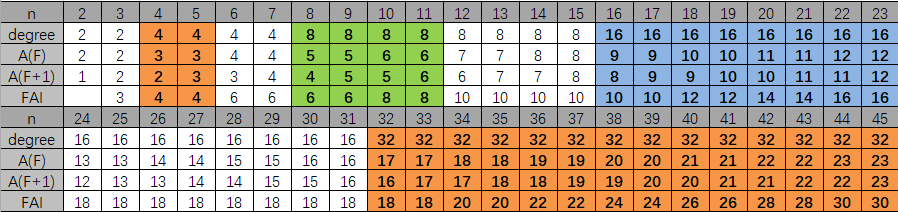
\includegraphics[width=1.0\linewidth]{computer-fai.jpg}  
		\caption{Research process}  
	\end{figure}
}

\section{Research Plan}
\frame {\frametitle{Research Plan}	
	\begin{itemize}
		\item Theoretical proof of the fast algebraic immunity of some special Boolean functions.
		\item [~] ~
		\item Security evaluation of block cipher for differential and linear cryptanalysis(MILP).
		\item [~] ~
		\item Sagemath
	\end{itemize}
}

\section{Reference}

\begin{thebibliography}{99}% more than 9 --> 99 / less than 10 --> 9
	
	
	\bibitem{Carlet2008} C.Carlet, K.Feng, An Infinite Class of Balanced Functions with Optimal Algebraic Immunity, Good Immunity to Fast Algebraic Attacks and Good Nonlinearity[C]// International Conference on the Theory and Application of Cryptology and Information Security: Advances in Cryptology. Springer-Verlag, 2008:425-440.
	
	\bibitem{Wang2010Constructions}Q.Wang, J.Peng, H.Kan, Constructions of Cryptographically Significant Boolean Functions Using Primitive Polynomials[J]. IEEE Transactions on Information Theory, 2010, 56(6):3048-3053.
	
		
	\bibitem{Chen2013}H.Chen, T.Tian, W.Qi, On the affine equivalence relation between two classes of Boolean functions with optimal algebraic immunity[J]. Designs Codes Cryptography, 2013, 67(2):175-185.
	
	\bibitem{Wang2010}Q.Wang, T.Johansson, On Equivalence Classes of Boolean Functions[M] Information Security and Cryptology - ICISC 2010. Springer Berlin Heidelberg, 2010:311-324.
	
		
	\bibitem{Meier2004} W. Meier, E. Pasalic, C. Carlet, "Algebraic attacks and decomposition of Boolean functions," International Conference on the Theory and Applications of Cryptographic Techniques, pp. 474-491, 2004.
	
	\bibitem{Liu2009fast} M. Liu, D. Lin, "Fast algebraic attacks and decomposition of symmetric Boolean functions," IEEE Trans. Inf. Theory, vol. 57, no. 7, pp. 4817-4821, 2011.
	
	\bibitem{Tang2014} D. Tang, C. Carlet, X. Tang, "A class of 1-resilient Boolean functions with optimal algebraic immunity and good behavior against fast algebraic attacks," International Journal of Foundations of Computer Science, vol. 25, no. 6, pp. 763-780, 2014.
	
	\bibitem{Tang2013} D. Tang, C. Carlet, X. Tang, "Highly nonlinear Boolean functions with optimal algebraic immunity and good behavior against fast algebraic attacks," IEEE Trans. Inf. Theory, vol. 59, no. 1, pp. 653-664, 2013.
		
	\bibitem{JinQ2011} Q. Jin, Z. Liu, B. Wu, "1-resilient Boolean function with optimal algebraic immunity," Cryptology ePrint Archive, Report 2011/549, http://eprint.iacr.org/.v

	\bibitem{Tang2016} D. Tang, R. Luo, and X. Du, "The exact fast algebraic immunity of two subclasses of the majority function," IEICE Trans. Fundamentals, vol. E99-A, no. 11, pp. 2084-2088, Nov. 2016.
	
	\bibitem{Ding1991}   C. Ding, G. Xiao, and W. Shan, "The stability theory of stream ciphers," (Lecture Notes in Computer Science), vol. 561, Springer Berlin Heidelberg, Berlin, Heidelberg, 1991.
	
	\bibitem{Dalai2006}    D.K. Dalai, S. Maitra, and S. Sarkar, "Basic theory in construction of Boolean functions with maximum possible annihilator immunity," Designs, Codes and Cryptography, vol. 40, no. 1, pp. 41-58, Jul. 2006.
	
	\bibitem{Armknecht2006}   F. Armknecht, C. Carlet, P. Gaborit, S. K\"{u}nzli, W.Meier, and O. Ruatta, "Efficient computation of algebraic immunity for algebraic and fast algebraic attacks," in Advances in Cryptology-EUROCRYPT, (Lecture Notes in Computer Science), vol. 4004, pp. 147-164, Springer Berlin Heidelberg, Berlin, Heidelberg, 2006.
	
	
	
\end{thebibliography}

\end{document}

